\scanpage{73}\mspage{72}

sous-figure de \deleted{$\unsure{G'|F'}$} la subdivision $F'$ de $F$, induite par la sous-figure $\deleted{F}G$ de $F$.
% slanted, upper-left margin
\margin{\unsure{double} \unsure{Transitivité} de l'induction}

$\uline{C}7_0$ Pour toute figure $F$, sous-figure $G$, et subdivision $G'$ de $G$, il existe une subdivision $F'$ de $F$ qui induise $\unsure{C'|G'}$\unsure{.|,}

(mais l'énoncé symétrique, où on échangerait les rôle de
% graphic: role-mark; the long stem continues the q above. Its worked foot
% does not securely establish a separate deleted l or F.
\unsure{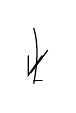
\begin{tikzpicture}[x=.035cm,y=.035cm,baseline=-.1ex,line width=.45pt,line cap=round]
\draw (5,20) .. controls (7,13) and (6,6) .. (5,0);
\draw (3,10) -- (3,3) -- (8,10);
\draw (4,4) -- (10,12);
\draw (5,1) -- (8,1);
\end{tikzpicture}}
$\leq$ et $\preceq$, est faux
% graphic: faux-mark; crossed upper curls, lower hook and rising arm.
\unsure{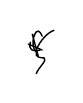
\begin{tikzpicture}[x=.025cm,y=.025cm,baseline=-.1ex,line width=.5pt,line cap=round,line join=round]
\draw (3,19) .. controls (4,23) and (6,22) .. (7,19);
\draw (3,20) .. controls (2,16) and (2,13) .. (4,11)
 .. controls (3,8) and (7,8) .. (8,8)
 .. controls (10,7) and (5,3) .. (4,0);
\draw (2,20) -- (5,9);
\draw (1,16) .. controls (0,12) and (2,11) .. (6,12);
\draw (0,15) -- (7,12);
\draw (4,12) .. controls (6,17) and (10,21) .. (13,22);
\end{tikzpicture}}
: il n'est pas vrai, pour $F'\preceq F$ donnés, que tte sous figure $G'$ de $F'$ \unsure{soit|sont} induite par une ss-figure $G$ de $\deleted{G}F$).

On \deleted{peut} renforcera par la suite $C7_0$ en
% graphic: before-c7; a small separate curved stroke, possibly an s or a
% worked beginning, with no secure independent cancellation line.
\unsure{\begin{tikzpicture}[x=.025cm,y=.025cm,baseline=-.1ex,line width=.45pt,line cap=round]
\draw (4,9) .. controls (5,6) and (3,5) .. (3,3)
 .. controls (3,2) and (1,1) .. (0,1);
\end{tikzpicture}}$C7$, en prenant un choix canonique de $F'$.

% figure: cancelled-draft
% All text in this group belongs to the draft cancelled by the THREE drawn
% oblique strokes. The heading has a separate scribbled cancellation;
% équivalentes and the C6 line have separate local strikes. The text occurs
% once, and the actual cancellation geometry supplies its deletion state.
\figure{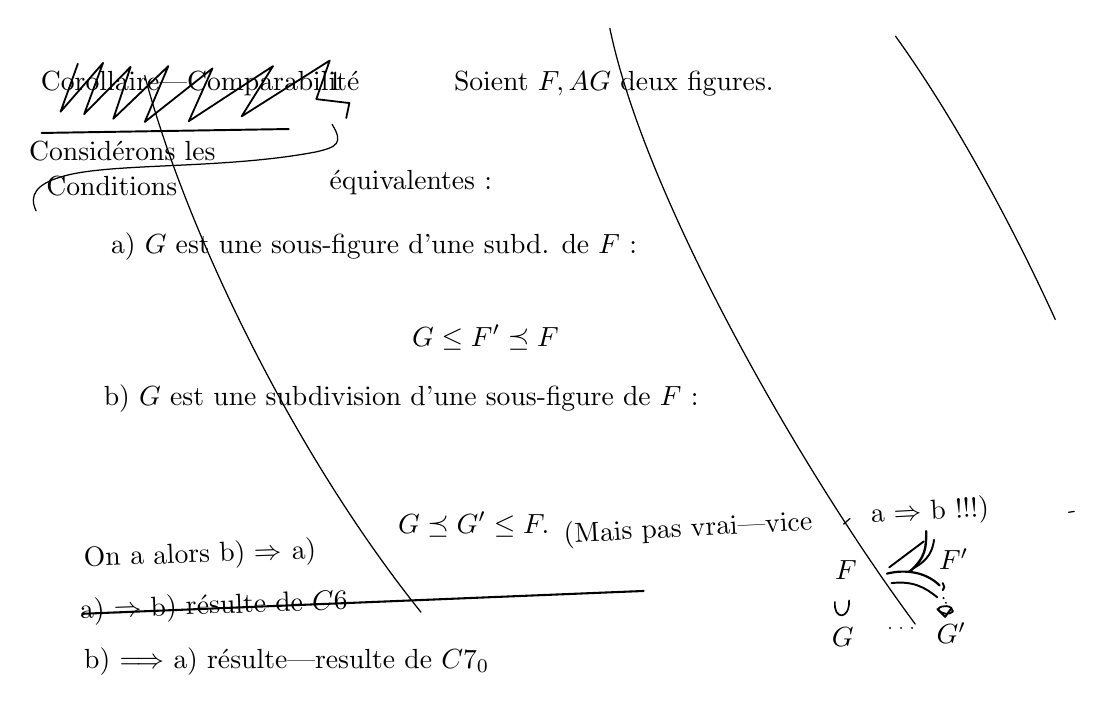
\begin{tikzpicture}[x=.01cm,y=-.01cm,line width=.45pt,line cap=round,line join=round,
 every node/.style={inner sep=0pt,outer sep=0pt,font=\normalsize}]
\node[anchor=base west] at (15,85) {\unsure{Corollaire|Comparabilité}};
\node[anchor=base west] at (380,85) {\unsure{1}};
\draw[line width=.7pt] (16,139) -- (330,134);
% The independent zigzag over the heading is not an extra unreadable word.
\draw[line width=.65pt] (62,51) -- (40,112) -- (94,50) -- (70,115)
 -- (129,55) -- (107,121) -- (177,54) -- (147,125)
 -- (233,57) -- (203,124) -- (310,54) -- (270,118)
 -- (382,47) -- (365,96) -- (407,101) -- (403,120);
\node[anchor=base west] at (540,85) {Soient $F,\deleted{A}G$ deux figures.};
\node[anchor=base west] at (0,174) {\inserted{Considérons les}};
\node[anchor=base west] at (22,218) {Conditions};
\node[anchor=base west] at (382,211) {\deleted{équivalentes} :};
% graphic: insertion-arm, an open enclosure beneath the entire raised phrase,
% returning to the beginning of Conditions; no supplied arrowhead.
\draw (385,128) .. controls (400,152) and (391,157) .. (365,163)
 .. controls (245,186) and (100,176) .. (40,195)
 .. controls (10,204) and (-1,218) .. (9,238);
\node[anchor=base west] at (104,292) {a) $G$ est une sous-figure d'une subd. de $F$ :};
\node[anchor=center] at (580,374) {\begin{minipage}{4cm}\[G\leq F'\preceq F\]\end{minipage}};
\node[anchor=base west,text width=12.4cm,align=left] at (95,485) {b) $G$ est une subdivision d'une sous-figure de $F$ :};
\node[anchor=center] at (565,612) {\begin{minipage}{4cm}\[G\preceq G'\leq F.\]\end{minipage}};
\node[anchor=base west,rotate=2] at (70,690) {On a alors b) $\Rightarrow$ a)};
\node[anchor=base west,rotate=3] at (680,660) {(Mais pas \unsure{vrai|vice}};
\node[anchor=base west,rotate=3] at (1070,634) {a $\Rightarrow$ b !!!)};
% graphic: conclusion-ticks; first merges with the long cancellation stroke,
% second touches the right closing parenthesis. Neither is forced to a stop.
\draw (1043,629) -- (1035,636);
\draw (1321,621) -- (1328,620);
\node[anchor=base west,rotate=2] at (65,756) {a) $\Rightarrow$ b) résulte de $C6$};
\draw[line width=.75pt] (68,750) -- (781,721);
\node[anchor=base west] at (70,819) {b) $\Longrightarrow$ a) \unsure{résulte|resulte} de $C7_0$};
% diagram: cancelled-draft/diagram. Positions, empty spaces and small marks
% are drawn literally; the worked top order is not normalized to a prime.
\node[anchor=center] at (1038,695) {$F$};
\node[anchor=center] at (1175,681) {$F'$};
\node[anchor=center] at (1034,780) {$G$};
\node[anchor=center] at (1172,775) {$G'$};
% Bowed relation with a second rising branch and taller hooked branch.
\draw[line width=.7pt] (1093,691) -- (1137,658);
\draw[line width=.8pt] (1090,699) .. controls (1114,693) and (1140,697) .. (1157,714);
\draw[line width=.7pt] (1096,711) .. controls (1123,708) and (1138,716) .. (1154,729);
\draw[line width=.85pt] (1118,697) .. controls (1140,679) and (1140,665) .. (1140,645);
\draw[line width=.7pt] (1124,692) .. controls (1144,681) and (1148,669) .. (1150,656);
\node[anchor=center] at (1134,683) {$\unsure{\phantom{\preceq}}$};
% Rounded cup at left; three separate bottom dots.
\draw[line width=.6pt] (1024,735) .. controls (1022,758) and (1043,758) .. (1042,733);
\fill (1094,768) circle[radius=1.35];
\fill (1108,768) circle[radius=1.35];
\fill (1122,768) circle[radius=1.35];
% Broken right edge and its worked, downward-pointing endpoint.
\draw[line width=.7pt] (1161,711) -- (1163,716) -- (1161,720);
\fill (1162,730) circle[radius=1.5];
\fill (1165,736) circle[radius=1.4];
\draw[line width=.7pt] (1154,744) -- (1164,754) -- (1172,743);
\draw[line width=.65pt] (1155,744) .. controls (1159,738) and (1174,739) .. (1174,747)
 .. controls (1171,751) and (1160,752) .. (1155,744);
% Complete broad cancellation: left, middle and shorter right stroke.
\draw (147,66) .. controls (198,259) and (333,542) .. (498,748);
\draw (738,6) .. controls (783,224) and (983,570) .. (1126,763);
\draw (1101,16) .. controls (1183,130) and (1257,273) .. (1304,376);
\end{tikzpicture}}
